\chapter{結果}
\label{chap:結果}

本章では，提案手法の有効性を Phase 1（対照学習）と Phase 2（強化学習）の順に検証する．
本章で示す主要な観察結果は以下の 3 点である．
\begin{enumerate}
  \item 対照学習で言語-動作対応が一定程度獲得されること
  \item 潜在空間から速度情報が統計的に復元可能であること
  \item 強化学習における補助速度条件下でのスタイル付与結果
\end{enumerate}


本章で可視化のために，4つのカテゴリを参照する場合，対応は
速い系（すたすた，せかせか，てくてく），
遅い系（とぼとぼ，のろのろ），
重い系（どっしどっし，のしのし），
ふらふら系（ぶらぶら，よたよた，よろよろ）
とする．

\subsection{埋め込みモデルの比較（Sarashina vs SigLIP）}
\label{subsec:embedding_compare}


\begin{figure}[htbp]
  \centering
  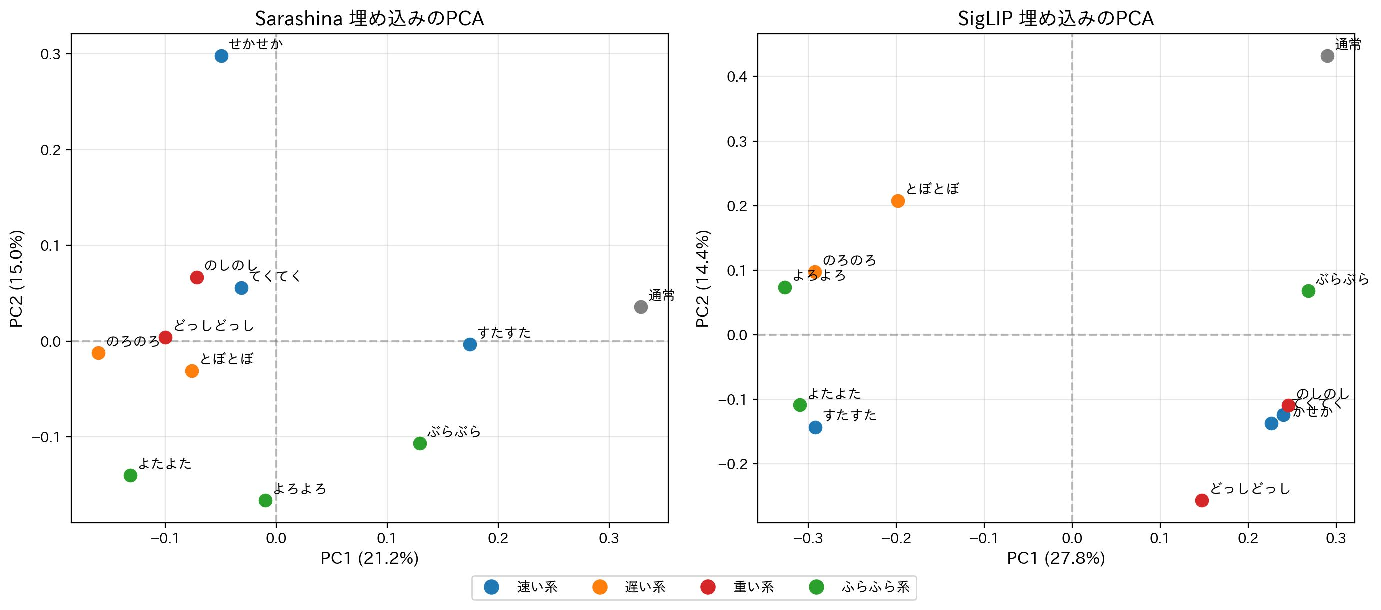
\includegraphics[width=0.9\linewidth]{figs/4/pca_comparison_sarashina_siglip.pdf}
  \caption{学習前のオノマトペ埋め込みの PCA 可視化（Sarashina vs SigLIP）}
  \label{fig:embedding_pca}
\end{figure}

図\ref{fig:embedding_pca}は，テンプレート文
\texttt{「<w>と歩いている．」} に対する埋め込みを PCA で 2 次元へ射影した結果である．
Sarashina は PC1/PC2 の寄与率が 21.16\%/14.96\%（累積 36.12\%），
SigLIP は 27.81\%/14.41\%（累積 42.22\%）であった．
可視化上は両者ともカテゴリ間の重なりが見られ，
学習前の埋め込みだけでは線形分離が明確に成立するわけではない．

ただし，速度の遅速に対応する連続的な並びは Sarashina の方が相対的に読み取りやすく，
通常が中央付近，せかせかが上側，よろよろが下側に配置される傾向が確認できた．
この配置は，PC2 軸が速度（歩行テンポ）の差を反映している可能性を示唆する．
この観察に基づき，本研究では対照学習の埋め込みモデルとして Sarashina を採用した．
なお，最終的な有効性は対照学習後の検索指標と潜在構造で判断する．

\subsection{対照学習の結果}
\label{subsec:contrastive_results}

Phase 1 の対照学習について，11 ラベル設定で
$\tau$，$\lambda_{\mathrm{vae}}$，$\lambda_{\mathrm{con}}$ をスイープし，seed を変えた複数回学習の
平均（mean$\pm$std）で性能を評価した．
評価指標は \ref{subsec:contrastive_metrics} 節の定義に従い，
$\mathrm{avg\_r@1}$ を主指標として報告する．
まず探索段階（Optuna）で有望領域を特定し，次に seed 平均の本番実験で再評価する．

\subsubsection{Optuna による探索結果}
\label{subsubsec:optuna_results}

Optuna（30 trials）により $\mathrm{avg\_r@1}$ を最大化する条件を探索した．
最良 trial（Trial 1）は $\mathrm{avg\_r@1}=0.611$ を達成し，
$\tau\approx 0.02$，$\lambda_{\mathrm{con}}=2.36$，$\lambda_{\mathrm{vae}}=0.057$ を選択した．
上位 trial の概要を表\ref{tab:optuna_top_trials}に示す．

\begin{table}[H]
  \centering
  \caption{Optuna における上位 trial（SupCon，検索再現率最大化）}
  \label{tab:optuna_top_trials}
  \begin{tabular}{cccccc} \toprule
    \textbf{Trial} & $\mathrm{avg\_r@1}$ & $\lambda_{\mathrm{con}}$ & $\lambda_{\mathrm{vae}}$ & $\tau$ & \textbf{特徴}           \\ \midrule
    1              & 0.611               & 2.36                     & 0.057                    & 0.021  & 高Cont / 低VAE / 低Temp \\
    12             & 0.573               & 1.09                     & 0.078                    & 0.020  & Cont中でも低Temp        \\
    13             & 0.557               & 2.20                     & 0.072                    & 0.059  & Temp高めだがバランス良  \\
    27             & 0.528               & 1.28                     & 0.230                    & 0.053  & VAE高めでも健闘         \\ \bottomrule
  \end{tabular}
\end{table}

上位 trial の比較から，以下の傾向が得られた．
\begin{itemize}
  \item \textbf{温度 $\tau$ の寄与が大きい}:\\
    上位 trial は共通して $\tau\approx 0.02$（探索下限付近）を選択した．
  \item \textbf{高 contrastive / 低 VAE が検索性能に有利}:\\
    $\lambda_{\mathrm{con}}$ を大きく（$>2$），
    $\lambda_{\mathrm{vae}}$ を小さく（$<0.1$）すると $\mathrm{avg\_r@1}$ が高くなる傾向が見られた．
  \item \textbf{VAE の強すぎる正則化は不利}:\\
    $\lambda_{\mathrm{vae}}$ を過度に大きくすると（例：$>0.2$），
    再構成誤差の最適化に寄りすぎ，言語-動作対応の精度が低下するトレードオフが確認された．
\end{itemize}

なお Optuna での指標は単一 seed・単一 val 分割に基づく参考値であり，
以降では，この探索結果を初期仮説として，本番実験の再現性を確認する．

\subsubsection{本番実験の結果（seed 平均）}
\label{subsubsec:contrastive_main_results}

本番実験では，fine（11 ラベル）設定のまま，
seed（41/42/43）を変えた複数試行の平均で評価した．
Optuna で得た有望領域を踏まえ，次の近傍条件を再評価した．
\begin{itemize}
  \item 温度：$\tau \in \{0.02,\,0.03,\,0.07,\,0.10\}$
  \item VAE 重み：$\lambda_{\mathrm{vae}} \in \{0.03,\,0.06,\,0.12\}$
  \item 対照損失重み：$\lambda_{\mathrm{con}} \in \{1.0,\,2.0,\,3.0\}$
\end{itemize}
再評価結果を表\ref{tab:contrastive_sweeps}，表\ref{tab:contrastive_best}に示す．


\begin{table}[H]
  \centering
  \caption{ハイパーパラメータごとの影響（seed 平均）}
  \label{tab:contrastive_sweeps}
  \begin{tabular}{llc} \toprule
    \textbf{スイープ}        & \textbf{条件}                                                          & $\mathrm{avg\_r@1}$ \\ \midrule
    temp                     & $\lambda_{\mathrm{con}}=2.0,\ \lambda_{\mathrm{vae}}=0.06,\ \tau=0.02$ & $0.346\ \pm\ 0.211$ \\
    temp                     & $\lambda_{\mathrm{con}}=2.0,\ \lambda_{\mathrm{vae}}=0.06,\ \tau=0.03$ & $0.328\ \pm\ 0.231$ \\
    temp                     & $\lambda_{\mathrm{con}}=2.0,\ \lambda_{\mathrm{vae}}=0.06,\ \tau=0.07$ & $0.316\ \pm\ 0.231$ \\
    temp                     & $\lambda_{\mathrm{con}}=2.0,\ \lambda_{\mathrm{vae}}=0.06,\ \tau=0.10$ & $0.214\ \pm\ 0.117$ \\
    \midrule
    $\lambda_{\mathrm{vae}}$ & $\lambda_{\mathrm{con}}=2.0,\ \tau=0.05,\ \lambda_{\mathrm{vae}}=0.03$ & $0.314\ \pm\ 0.174$ \\
    $\lambda_{\mathrm{vae}}$ & $\lambda_{\mathrm{con}}=2.0,\ \tau=0.05,\ \lambda_{\mathrm{vae}}=0.06$ & $0.302\ \pm\ 0.190$ \\
    $\lambda_{\mathrm{vae}}$ & $\lambda_{\mathrm{con}}=2.0,\ \tau=0.05,\ \lambda_{\mathrm{vae}}=0.12$ & $0.356\ \pm\ 0.224$ \\
    \midrule
    $\lambda_{\mathrm{con}}$ & $\lambda_{\mathrm{vae}}=0.06,\ \tau=0.05,\ \lambda_{\mathrm{con}}=1.0$ & $0.334\ \pm\ 0.248$ \\
    $\lambda_{\mathrm{con}}$ & $\lambda_{\mathrm{vae}}=0.06,\ \tau=0.05,\ \lambda_{\mathrm{con}}=2.0$ & $0.302\ \pm\ 0.190$ \\
    $\lambda_{\mathrm{con}}$ & $\lambda_{\mathrm{vae}}=0.06,\ \tau=0.05,\ \lambda_{\mathrm{con}}=3.0$ & $0.285\ \pm\ 0.202$ \\ \bottomrule
  \end{tabular}
\end{table}

\begin{table}[H]
  \centering
  \caption{対照学習（fine）のベスト設定（seed 平均）}
  \label{tab:contrastive_best}
  \begin{tabular}{lccccc} \toprule
    $\lambda_{\mathrm{con}}$ & $\lambda_{\mathrm{vae}}$ & $\tau$ & $\mathrm{m2t\_r@1}$ & $\mathrm{t2m\_r@1}$ & $\mathrm{avg\_r@1}$ \\ \midrule
    2.0                      & 0.12                     & 0.05   & $0.258\ \pm\ 0.168$ & $0.455\ \pm\ 0.282$ & $0.356\ \pm\ 0.224$ \\ \bottomrule
  \end{tabular}
\end{table}

さらに，採用設定
（$\lambda_{\mathrm{con}}=2.0,\ \lambda_{\mathrm{vae}}=0.12,\ \tau=0.05$）
において，$\mathrm{avg\_r@1}$ が最大となった checkpoint
（seed=43，step=4600）の詳細指標を表\ref{tab:contrastive_best_checkpoint}に示す．

\begin{table}[H]
  \centering
  \caption{対照学習 best model の性能（採用設定内の最良 checkpoint）}
  \label{tab:contrastive_best_checkpoint}
  \begin{tabular}{lc} \toprule
    \textbf{指標} & \textbf{best model} \\ \midrule
    M2T R@1       & 0.468               \\
    M2T R@3       & 0.758               \\
    M2T R@5       & 0.871               \\
    T2M R@1       & 0.818               \\
    T2M R@3       & 0.909               \\
    T2M R@5       & 0.909               \\
    avg R@1       & 0.643               \\
    Silhouette    & -0.020              \\ \bottomrule
  \end{tabular}
\end{table}

表\ref{tab:contrastive_sweeps}より，以下の傾向が観察された．
\begin{itemize}
  \item 温度 $\tau$ は検索性能に対する影響が最も大きく，
        高温（$\tau=0.10$）で性能が明確に低下した．
  \item $\tau=0.02$〜0.07 では平均値の差が比較的小さく，低温側がやや優位であった．
  \item $\lambda_{\mathrm{vae}}=0.12$ で平均性能が最も高かった．
  \item $\lambda_{\mathrm{con}}=3.0$ では平均性能が低下し，試行間分散が増加した．
\end{itemize}
以上より，本研究の設定では温度 $\tau$ の影響が最も支配的であり，
contrastive と VAE の重みはその次に効く調整軸であることが確認された．
この中で，$\lambda_{\mathrm{con}}=2.0,\ \lambda_{\mathrm{vae}}=0.12,\ \tau=0.05$ を
best model（最良モデル）として採用した（表\ref{tab:contrastive_best}）．
同条件のシルエット係数は $-0.212 \pm 0.201$であった．

\subsubsection{可視化}
\label{subsubsec:contrastive_visualization}

学習中の損失推移を図\ref{fig:contrastive_loss_curve}に，
検索指標（R@1）の推移を図\ref{fig:contrastive_metrics_curve}に示す．
freeze 段階では encoder を凍結してテキスト側のみを学習し，
full 段階で encoder を含めた fine-tuning を行った．
以下の可視化は，前節で採用した best model
（$\lambda_{\mathrm{con}}=2.0,\ \lambda_{\mathrm{vae}}=0.12,\ \tau=0.05$）に基づく．

\begin{figure}[H]
  \centering
  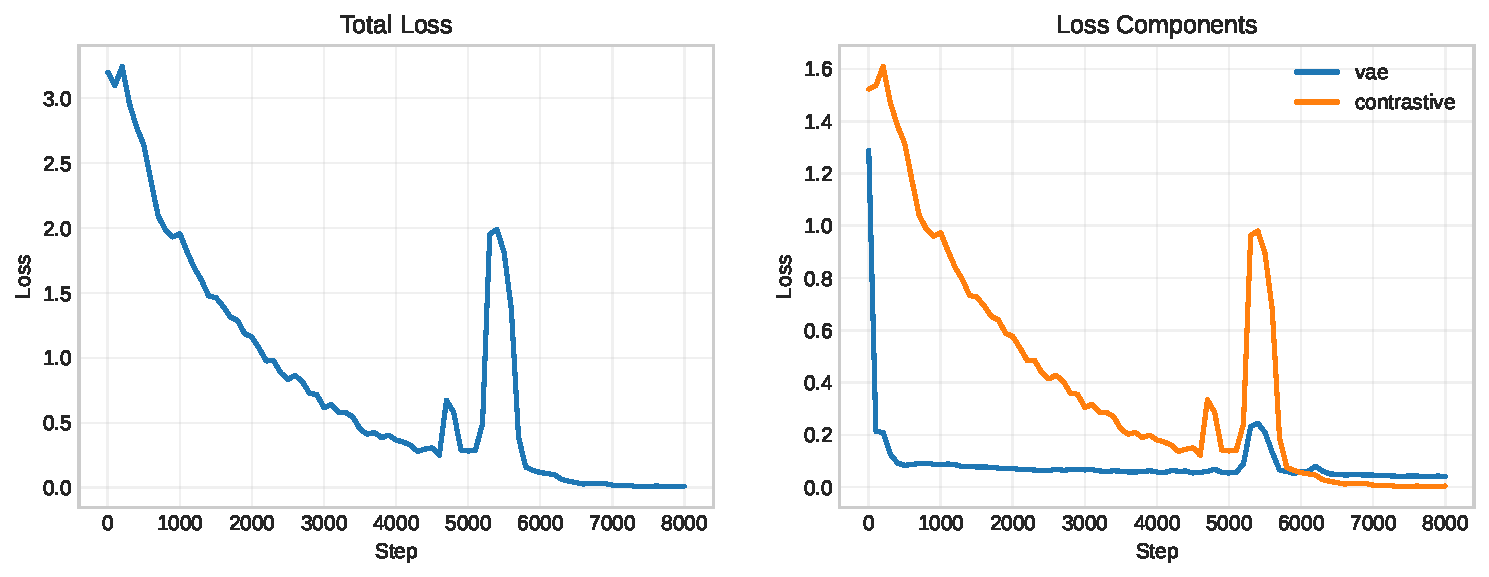
\includegraphics[width=0.95\linewidth]{figs/4/contrastive_loss_curve.pdf}
  \caption{対照学習における損失推移（freeze / full）}
  \label{fig:contrastive_loss_curve}
\end{figure}

\begin{figure}[H]
  \centering
  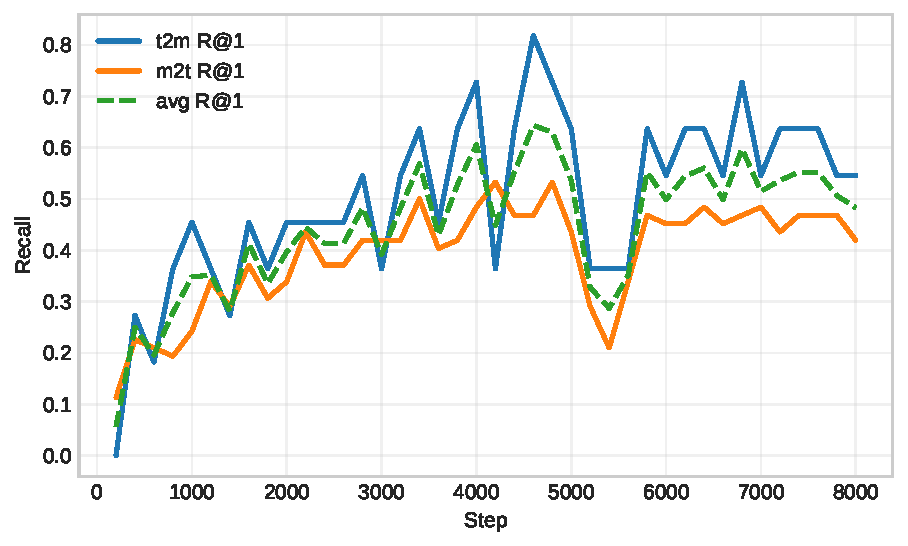
\includegraphics[width=0.95\linewidth]{figs/4/contrastive_metrics_curve.pdf}
  \caption{検索指標 R@1 の推移（freeze / full）}
  \label{fig:contrastive_metrics_curve}
\end{figure}

図\ref{fig:contrastive_pca_fine}に通常＋4カテゴリ（速い系・遅い系・重い系・ふらふら系）で色分けした埋め込み PCA を示す．
図\ref{fig:contrastive_pca_fine}は学習ラベルを 5 カテゴリに集約した可視化であり，未知語は含まない．
また，図\ref{fig:contrastive_pca_unknown}に未知語（学習時に含まれなかったオノマトペ）を重ねた PCA 可視化を示す．
未知語のテキストプロトタイプは，意味的に近い学習ラベルの近傍に配置される傾向が確認できる．
PCA 上ではクラス間の重なりが残っており，シルエット係数は負であった．
すなわち，潜在空間は完全分離には至らない一方で，局所的な近傍構造は保持されていると解釈できる．

\begin{figure}[H]
  \centering
  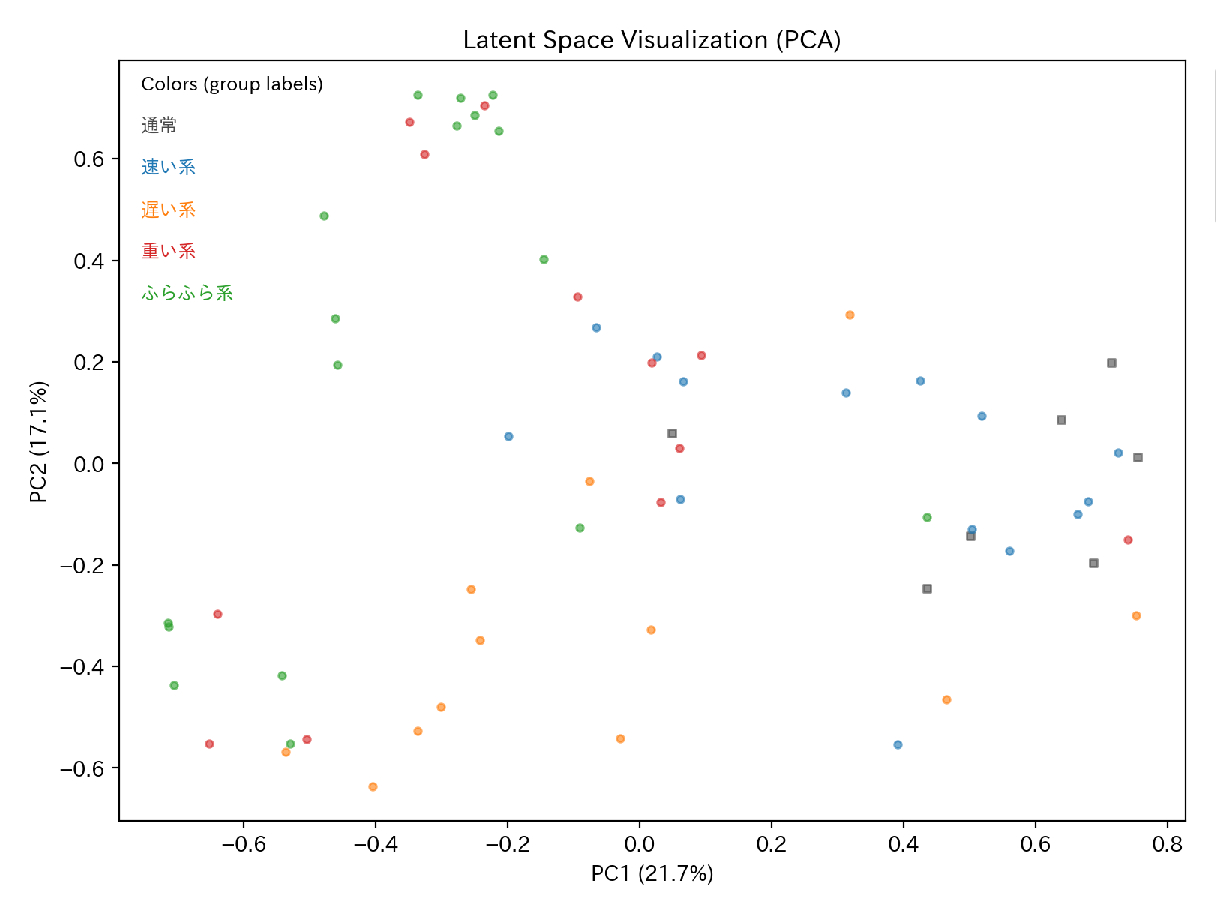
\includegraphics[width=0.85\linewidth]{figs/4/contrastive_latent_pca_fine.pdf}
  \caption{埋め込みの PCA 可視化（通常＋4カテゴリ，凡例付き）}
  \label{fig:contrastive_pca_fine}
\end{figure}

\begin{figure}[H]
  \centering
  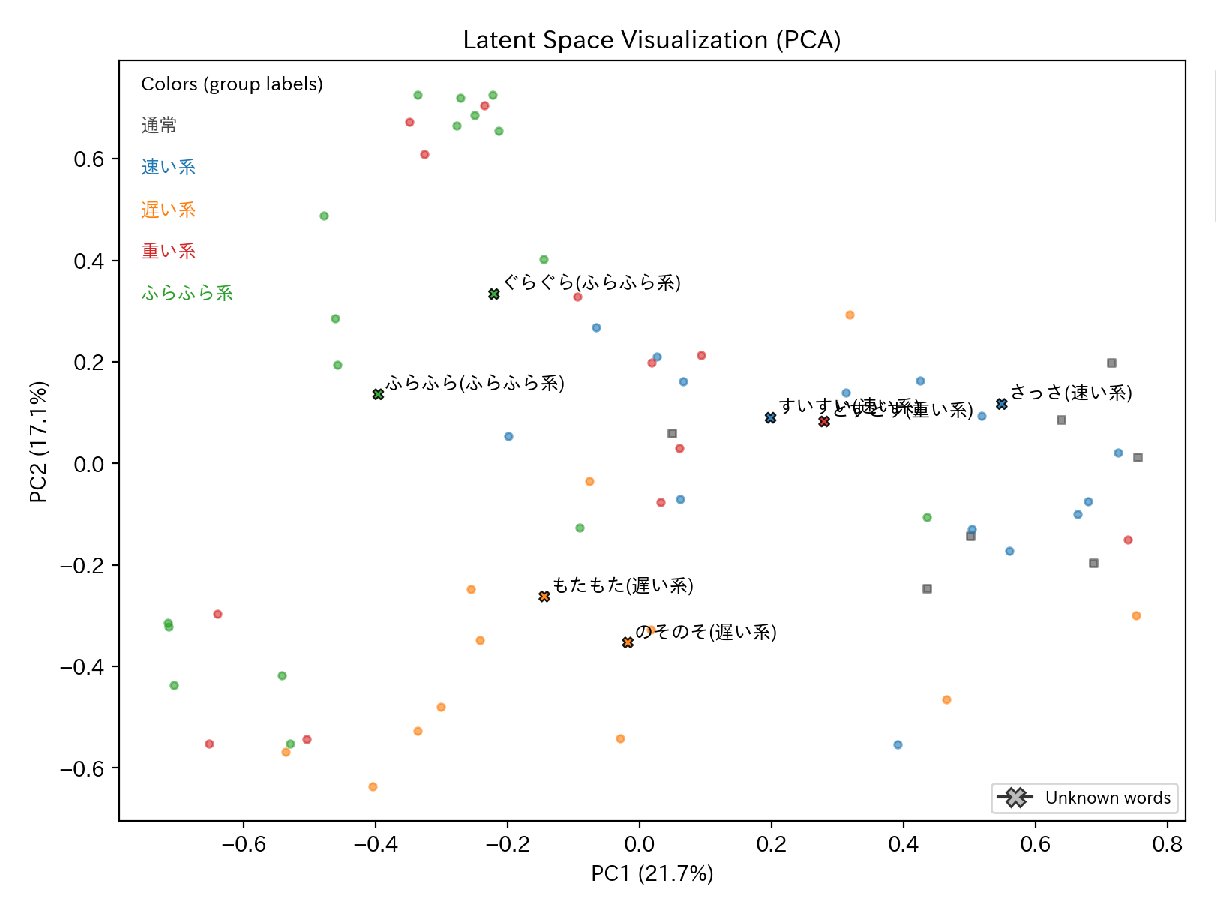
\includegraphics[width=0.85\linewidth]{figs/4/contrastive_latent_pca_fine_unknown.pdf}
  \caption{埋め込みの PCA 可視化（未知語を含む，通常＋4カテゴリで色分け）}
  \label{fig:contrastive_pca_unknown}
\end{figure}



\begin{figure}[H]
  \centering
  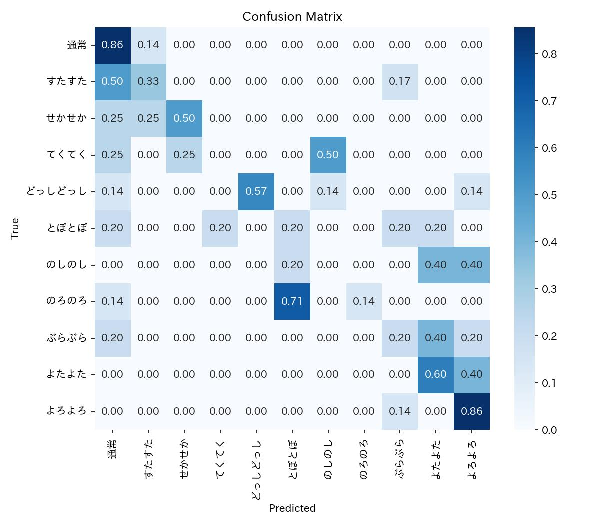
\includegraphics[width=0.85\linewidth]{figs/4/contrastive_confusion_fine.pdf}
  \caption{Motion$\rightarrow$Textの混同行列}
  \label{fig:contrastive_confusion_fine}
\end{figure}

\begin{figure}[H]
  \centering
  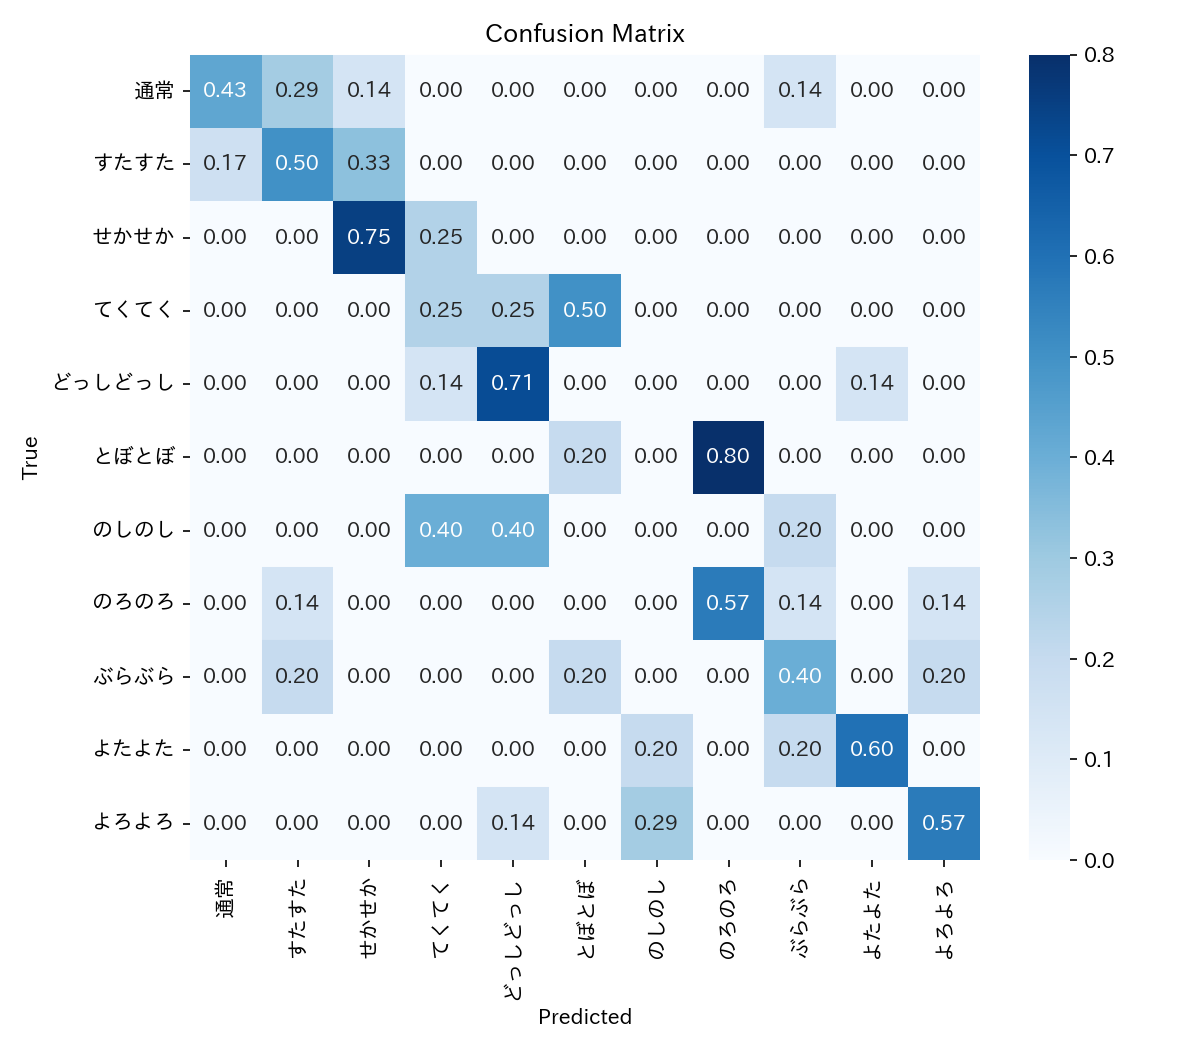
\includegraphics[width=0.85\linewidth]{figs/4/contrastive_confusion_t2m_fine.pdf}
  \caption{Text$\rightarrow$Motionの混同行列}
  \label{fig:contrastive_confusion_t2m_fine}
\end{figure}

図\ref{fig:contrastive_confusion_fine}に Motion$\rightarrow$Text の混同行列を示し，
図\ref{fig:contrastive_confusion_t2m_fine}に Text$\rightarrow$Motion の混同行列を示す．
混同行列では対角成分が相対的に高く，言語-動作対応が一定程度成立していることが分かる．
一方で，遅い系どうし，ふらふら系どうしなど意味が近いスタイル間で非対角成分が残り，
境界付近の取り違えが生じている．
この結果は，潜在空間がカテゴリ間を大局的には分離しつつも，
局所的には連続的な意味構造を保持していることを示唆する．



\subsubsection{潜在空間における速度情報の反映}
\label{subsubsec:contrastive_speed_reflection}

第\ref{subsec:contrastive_speed_reflection_eval}節の評価プロトコルに基づき，
best model の潜在空間における速度反映の評価結果を
表\ref{tab:contrastive_speed_reflection_metrics}に示す．

\begin{table}[H]
  \centering
  \caption{潜在速度反映の評価結果（best model，$N=284$，5-fold OOF，permutation=1000）}
  \label{tab:contrastive_speed_reflection_metrics}
  \begin{tabular}{lc} \toprule
    \textbf{指標} & \textbf{best model} \\ \midrule
    Spearman $\rho$ & 0.907 \\
    回帰 $R^2$ & 0.835 \\
    回帰 MAE & 0.007 \\
    3分位分類 macro-F1 & 0.844 \\
    3分位分類 balanced acc & 0.854 \\
    Permutation $p$（$\rho$） & ${<}\,0.001$ \\
    Permutation $p$（macro-F1） & ${<}\,0.001$ \\
    \bottomrule
  \end{tabular}
\end{table}

速度代理指標 $v_{\mathrm{scale}}$ の算出に用いた HOYO 側の相対速度マッピングを
表\ref{tab:hoyo_relative_speed_table}に示す．
各値は，$p90$ raw 速度の最大値を 1.00 とした相対値である\footnote{基準値 $p90\ \mathrm{raw}=0.020842$．}．

\begin{table}[H]
  \centering
  \caption{HOYO 相対速度テーブル}
  \label{tab:hoyo_relative_speed_table}
  \begin{tabular}{lc} \toprule
    \textbf{オノマトペ} & \textbf{相対速度 [x]} \\ \midrule
    すたすた & 1.000 \\
    せかせか & 1.000 \\
    てくてく & 0.708 \\
    とぼとぼ & 0.428 \\
    どっしどっし & 0.699 \\
    のしのし & 0.511 \\
    のろのろ & 0.448 \\
    ぶらぶら & 0.567 \\
    よたよた & 0.466 \\
    よろよろ & 0.274 \\
    通常 & 0.892 \\ \bottomrule
  \end{tabular}
\end{table}

\noindent ここで \texttt{speed\_scale} は 2D 関節から算出した速度代理指標であり，
各サンプルの head--mid\_feet 距離 $h_t$ に対して
$\log h_t$ の時間トレンドを最小二乗直線で近似した傾き
（負値は 0 にクリップ）として定義する．
したがって単位は m/s ではなく，カメラ奥行き方向の相対的なスケール変化率（1/s）である．

\begin{figure}[H]
  \centering
  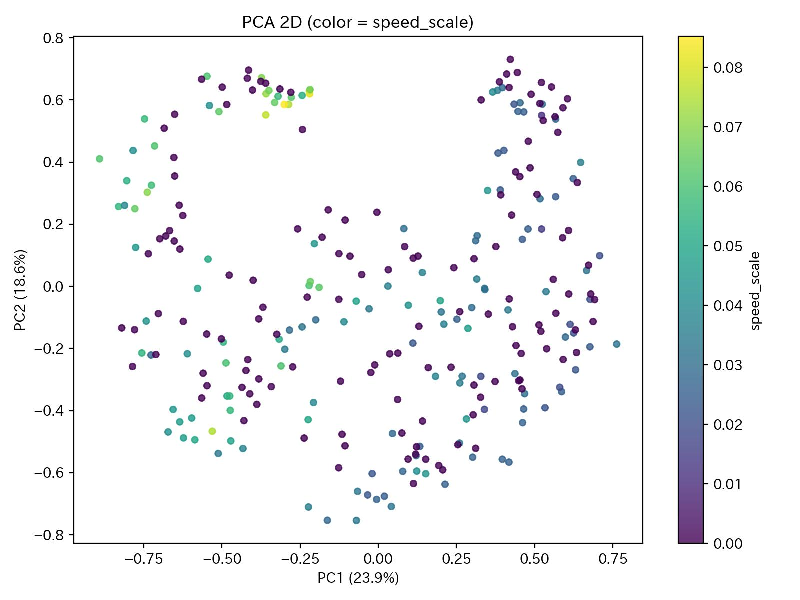
\includegraphics[width=0.72\linewidth]{figs/4/latent_speed_pca_new.pdf}
  \caption{潜在空間の PCA 可視化（raw \texttt{speed\_scale} による速度着色）．}
  \label{fig:contrastive_speed_pca_comparison}
\end{figure}

\begin{figure}[H]
  \centering
  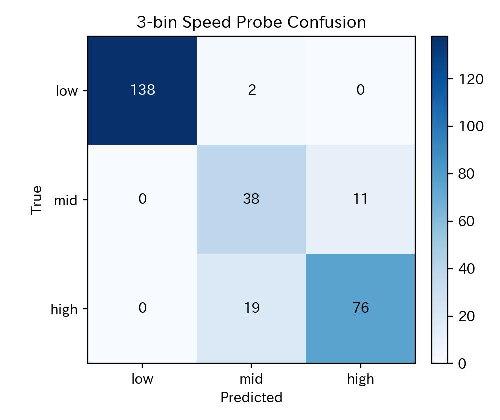
\includegraphics[width=0.62\linewidth]{figs/4/latent_speed_bin_confusion_new.pdf}
  \caption{3分位速度分類の混同行列（bin0=low，bin1=med，bin2=high）．速度帯の分離傾向が確認できる．}
  \label{fig:contrastive_speed_bin_confusion_comparison}
\end{figure}

表\ref{tab:contrastive_speed_reflection_metrics}より，
すべての指標が事前に定めた判定基準（$\rho \ge 0.35$，macro-F1 $\ge 0.50$，$p<0.05$）を
満たしており，潜在空間から速度情報が復元可能であることを確認した．
図\ref{fig:contrastive_speed_pca_comparison}の PCA 可視化でも
速度勾配に沿った連続的な配置が見て取れ，
図\ref{fig:contrastive_speed_bin_confusion_comparison}の混同行列でも
3 群間の分離傾向が確認できる\footnote{%
  3 群の境界は $v_{\mathrm{scale}}$ の 3 分位点で決定した．
  具体的には bin0=low（${\le}\,0.0$，$n{=}140$），
  bin1=med（$0.0\text{--}0.029$，$n{=}49$），
  bin2=high（${>}\,0.029$，$n{=}95$）である．}．

ただし，本評価はあくまで潜在空間に速度成分が含まれるかの確認であり，
速度を因果的に符号化していることや，RL 性能向上を直接保証するものではない．

\subsubsection{先行研究（MotionCLIP）との比較と考察}
\label{subsubsec:contrastive_prior_comparison}

MotionCLIP \cite{MotionCLIP} では，BABEL-60 を用いた行動認識実験として，
Top-1/Top-5 精度が報告されている（比較対象: 2s-AGCN \cite{agcn2s}, BABEL \cite{babel}）．
MotionCLIP 側も別途の分類器ヘッドを追加学習するのではなく，
クラス名埋め込みとの cosine 類似度（+ softmax）で分類している．
これに対し本研究では，motion$\rightarrow$text 検索の
$\mathrm{m2t\_R@}K$ を分類近似として評価した．
表\ref{tab:motionclip_comparison}に，先行研究値と本研究値の参考比較を示す．

\begin{table}[H]
  \centering
  \caption{先行研究（MotionCLIP）と本研究の参考比較}
  \label{tab:motionclip_comparison}
  \begin{tabular}{lcc} \toprule
    \textbf{手法 / 条件} & \textbf{Top-1 相当} & \textbf{Top-5 相当} \\ \midrule
    MotionCLIP（BABEL-60, 3D）              & 40.90\%               & 57.71\%               \\
    2s-AGCN（BABEL-60, 3D）                & 41.14\%               & 73.18\%               \\
    Ours（HOYO-11, 2D, seed平均）          & $40.32 \pm 1.32$\%    & $86.02 \pm 2.74$\%    \\
    Ours（HOYO-11, 2D, best単発）          & 41.94\%               & 88.71\%               \\ \bottomrule
  \end{tabular}
\end{table}

なお，本研究は分類器学習ではなく，motion$\rightarrow$text 検索（$\mathrm{m2t\_R@}K$）を
分類の近似として使用している．
そのため，表\ref{tab:motionclip_comparison}はあくまで参考比較として解釈する必要がある．

Top-1 相当値は，見かけ上 MotionCLIP と近い水準を示した．
ただし，以下の三点から厳密な性能比較は困難である．
%
\begin{itemize}
  \item データセットとクラス数が異なる（BABEL-60 vs HOYO-11）
  \item 入力の情報量が異なる（3D 関節表現 vs 2D 関節表現）
  \item 評価プロトコルが異なる（クラス名類似度に基づく分類 vs 検索近似）
\end{itemize}
%
Top-5 相当値についても，クラス数の差（60 vs 11）の影響が大きい．
以上を踏まえ，本節の主張は
\textbf{2D・小規模条件でも，言語と動作の意味整合を一定程度獲得できた}
という点に留まる．


\subsection{強化学習の結果}
\label{subsec:rl_results}

\noindent 本節では，強化学習結果を速度挙動（相対差）・安定性，スタイル識別，
およびオノマトペ別指標（速度・cos 類似度・関節誤差）に分けて整理する．
比較条件は主に $v_x^{\mathrm{cmd}}=0.5$ である.

本章では結果の提示に留め，未解決課題や要因分析は第\ref{chap:考察}章で扱う．
先に結論を述べると，補助速度条件 $v_x^{\mathrm{cmd}}=0.5$ に対する実速度は条件依存で乖離する一方，
語彙間には相対速度差と類似度差が観測され，オノマトペごとの見た目の違いが一部確認された．
ただし，スタイル識別の分離度にはなお改善余地が残った．

\subsubsection{速度挙動と安定性（速度指令値 0.5）}
\label{subsubsec:rl_results_20260201}

本小節では，以下のA/B/C/D の 4 条件を
$v_x^{\mathrm{cmd}}=0.5$ で比較する．

\begin{table}[htb]
  \centering
  \caption{強化学習比較で用いた条件と評価設定}
  \label{tab:rl_comparison_runs}
  \small
  \begin{tabular}{lll} \toprule
    \textbf{条件 ID} & \textbf{スタイル重み} & \textbf{速度条件} \\ \midrule
    A & 0.0 & $v_x^{\mathrm{cmd}}=0.5$ \\
    B & 2.0 & $v_x^{\mathrm{cmd}}=0.5$ \\
    C & 4.0 & $v_x^{\mathrm{cmd}}=0.5$ \\
    D & 6.0 & $v_x^{\mathrm{cmd}}=0.5$ \\
    \bottomrule
  \end{tabular}
\end{table}


条件ごとの平均指標を表\ref{tab:rl_abcd_main_m2999}に，
オノマトペ別の動力学系指標を表\ref{tab:rl_ab_onom_dynamics}および表\ref{tab:rl_cd_onom_dynamics}に，
オノマトペ別の類似度指標を表\ref{tab:rl_abcd_onom_similarity}に示す．

\begin{table}[H]
  \centering
  \caption{A/B/C/D 主比較（速度指令値 0.5）の平均指標}
  \label{tab:rl_abcd_main_m2999}
  \begin{tabular}{lcccc} \toprule
    \textbf{指標} & \textbf{A} & \textbf{B} & \textbf{C} & \textbf{D} \\ \midrule
    平均速度 $v_x$ & 0.4782 & 0.4511 & 0.2602 & 0.5027 \\
    速度 MAE（速度指令値比） & 0.0218 & 0.0489 & 0.2398 & 0.0027 \\
    転倒率 & 0.0000 & 0.0000 & 0.0000 & 0.0000 \\
    平均エピソード長 & 500.0 & 500.0 & 500.0 & 500.0 \\
    平均関節誤差 & 3.4624 & 3.5525 & 4.2470 & 3.7735 \\
    \bottomrule
  \end{tabular}
\end{table}

表\ref{tab:rl_abcd_main_m2999}より，補助速度条件を $v_x^{\mathrm{cmd}}=0.5$ に固定しても，
平均速度は条件間で 0.2602（C）〜0.5027（D）と大きく分かれた．
また，C 条件ではオノマトペ別速度が 0.1721〜0.3179
（表\ref{tab:rl_cd_onom_dynamics}）に分布しており，
絶対値としての速度一致よりも，語彙・条件に応じた相対的な速度差と
オノマトペらしい見え方の対応を
スタイル反映の観測対象として捉える必要がある．

\begin{table}[H]
  \centering
  \caption{オノマトペ別動力学系指標（A/B，速度指令値 0.5）}
  \label{tab:rl_ab_onom_dynamics}
  \small
  \setlength{\tabcolsep}{3.5pt}
  \begin{tabular}{lccc ccc} \toprule
    \textbf{オノマトペ} &
    \multicolumn{3}{c}{\textbf{A}} &
    \multicolumn{3}{c}{\textbf{B}} \\ \cmidrule(lr){2-4}\cmidrule(lr){5-7}
    & $v_x$ & fall & Err & $v_x$ & fall & Err \\ \midrule
    通常 & 0.4763 & 0.0000 & 2.6495 & 0.4295 & 0.0000 & 3.2371 \\
    すたすた & 0.4746 & 0.0000 & 4.0567 & 0.4503 & 0.0000 & 3.7675 \\
    せかせか & 0.4756 & 0.0000 & 3.1345 & 0.4593 & 0.0000 & 3.3808 \\
    てくてく & 0.4808 & 0.0000 & 3.0223 & 0.4157 & 0.0000 & 3.1164 \\
    どっしどっし & 0.4788 & 0.0000 & 3.2593 & 0.3906 & 0.0000 & 2.8458 \\
    とぼとぼ & 0.4785 & 0.0000 & 3.7722 & 0.4899 & 0.0000 & 4.1906 \\
    のしのし & 0.4833 & 0.0000 & 3.9135 & 0.4172 & 0.0000 & 4.2879 \\
    のろのろ & 0.4845 & 0.0000 & 3.1986 & 0.4545 & 0.0000 & 2.9634 \\
    ぶらぶら & 0.4777 & 0.0000 & 4.1924 & 0.4842 & 0.0000 & 4.4385 \\
    よたよた & 0.4808 & 0.0000 & 4.1211 & 0.4840 & 0.0000 & 3.7968 \\
    よろよろ & 0.4696 & 0.0000 & 2.7659 & 0.4870 & 0.0000 & 3.0531 \\
    \bottomrule
  \end{tabular}
\end{table}

\begin{table}[H]
  \centering
  \caption{オノマトペ別動力学系指標（C/D，速度指令値 0.5）}
  \label{tab:rl_cd_onom_dynamics}
  \small
  \setlength{\tabcolsep}{3.5pt}
  \begin{tabular}{lccc ccc} \toprule
    \textbf{オノマトペ} &
    \multicolumn{3}{c}{\textbf{C}} &
    \multicolumn{3}{c}{\textbf{D}} \\ \cmidrule(lr){2-4}\cmidrule(lr){5-7}
    & $v_x$ & fall & Err & $v_x$ & fall & Err \\ \midrule
    通常 & 0.2530 & 0.0000 & 4.2928 & 0.4912 & 0.0000 & 2.8579 \\
    すたすた & 0.3179 & 0.0000 & 3.9590 & 0.4571 & 0.0000 & 4.2372 \\
    せかせか & 0.2661 & 0.0000 & 4.3799 & 0.4602 & 0.0000 & 3.3877 \\
    てくてく & 0.2797 & 0.0000 & 4.1843 & 0.4836 & 0.0000 & 3.4234 \\
    どっしどっし & 0.2431 & 0.0000 & 4.1986 & 0.5228 & 0.0000 & 3.4436 \\
    とぼとぼ & 0.2411 & 0.0000 & 4.2839 & 0.5180 & 0.0000 & 4.0845 \\
    のしのし & 0.1721 & 0.0000 & 4.3083 & 0.5201 & 0.0000 & 4.4132 \\
    のろのろ & 0.2730 & 0.0000 & 4.1939 & 0.5032 & 0.0000 & 3.4331 \\
    ぶらぶら & 0.2921 & 0.0000 & 4.3407 & 0.5182 & 0.0000 & 4.3665 \\
    よたよた & 0.2700 & 0.0000 & 4.0734 & 0.5235 & 0.0000 & 4.4291 \\
    よろよろ & 0.2538 & 0.0000 & 4.5022 & 0.5317 & 0.0000 & 3.4328 \\
    \bottomrule
  \end{tabular}
\end{table}

\begin{table}[t]
  \centering
  \caption{オノマトペごとの速度指標比較（通常=1で正規化）}
  \label{tab:onomatope_metrics}
  \small
  \setlength{\tabcolsep}{4pt}
  \begin{tabular}{lcccc}
    \hline
    オノマトペ & $v_x$ & $v_x$の相対速度 & 教師の相対速度 & $|相対速度の差分|$ \\
    \hline
    通常         & 0.253 & 1.000 & 1.000 & 0.000 \\
    すたすた     & 0.318 & 1.257 & 1.121 & 0.136 \\
    せかせか     & 0.266 & 1.051 & 1.121 & 0.070 \\
    てくてく     & 0.280 & 1.107 & 0.794 & 0.313 \\
    どっしどっし & 0.243 & 0.960 & 0.784 & 0.177 \\
    とぼとぼ     & 0.241 & 0.953 & 0.480 & 0.473 \\
    のしのし     & 0.172 & 0.680 & 0.573 & 0.107 \\
    のろのろ     & 0.273 & 1.079 & 0.502 & 0.577 \\
    ぶらぶら     & 0.292 & 1.154 & 0.636 & 0.518 \\
    よたよた     & 0.270 & 1.067 & 0.522 & 0.545 \\
    よろよろ     & 0.254 & 1.004 & 0.307 & 0.697 \\
    \hline
  \end{tabular}
\end{table}

\begin{table}[t]
  \centering
  \caption{オノマトペごとのその他指標比較}
  \label{tab:onomatope_other_metrics}
  \small
  \setlength{\tabcolsep}{4pt}
  \begin{tabular}{lccc}
    \hline
    オノマトペ & 転倒率 & Err & 類似度 \\
    \hline
    通常         & 0.000 & 4.29 & 0.471 \\
    すたすた     & 0.000 & 3.96 & 0.513 \\
    せかせか     & 0.000 & 4.38 & 0.483 \\
    てくてく     & 0.000 & 4.18 & 0.459 \\
    どっしどっし & 0.000 & 4.20 & 0.523 \\
    とぼとぼ     & 0.000 & 4.28 & 0.454 \\
    のしのし     & 0.000 & 4.31 & 0.422 \\
    のろのろ     & 0.000 & 4.19 & 0.451 \\
    ぶらぶら     & 0.000 & 4.34 & 0.563 \\
    よたよた     & 0.000 & 4.07 & 0.437 \\
    よろよろ     & 0.000 & 4.50 & 0.660 \\
    \hline
  \end{tabular}
\end{table}

A/B/D 条件では語彙間の速度差が小さく，
速い語と遅い語の序列が明確に現れているとは言い難い．
特に A 条件はスタイル報酬を与えていないモデルであり，
語彙によらずほぼ一様な速度に収束している．
これに対して C 条件（style\_weight=4.0）では，
補助速度条件への一致は弱まる代わりに語彙間の速度差が拡大しており，
たとえば「すたすた」が相対的に速く「のしのし」が遅いなど，
オノマトペの印象に沿った傾向が一部の語彙で確認できた．
ただし，すべての語彙で一貫した序列が得られたわけではない．
図\ref{fig:rl_sekaseka_sequence}に C 条件の「せかせか」実行動画から，
1歩行周期を6分割して抽出した連続フレームを示す．
同図では，周期内で左右脚の位相が遷移しつつ前進を維持する様子が確認でき，
C 条件で観測された語彙依存の速度差を見た目として補足している．

\begin{figure}[H]
  \centering
  \begin{subfigure}[t]{0.48\linewidth}
    \centering
    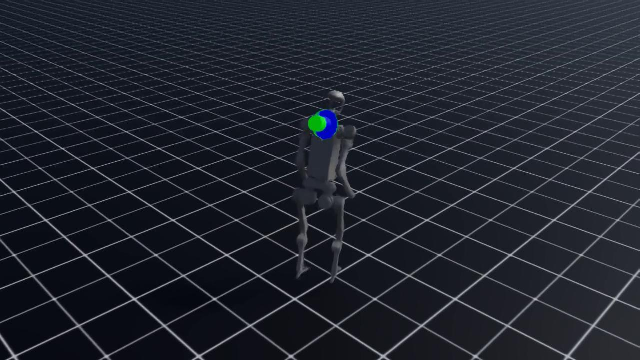
\includegraphics[width=\linewidth]{figs/5/sekaseka_seq_01.pdf}
  \end{subfigure}
  \hfill
  \begin{subfigure}[t]{0.48\linewidth}
    \centering
    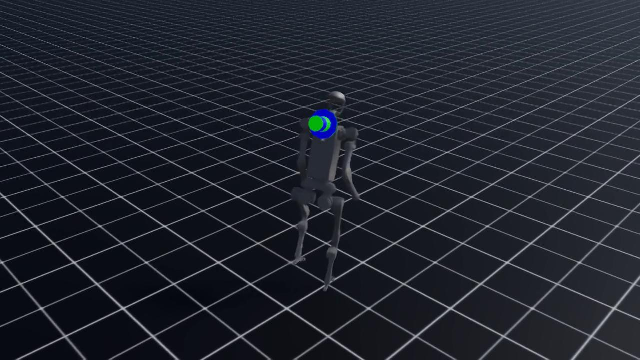
\includegraphics[width=\linewidth]{figs/5/sekaseka_seq_02.pdf}
  \end{subfigure}

  \vspace{1mm}

  \begin{subfigure}[t]{0.48\linewidth}
    \centering
    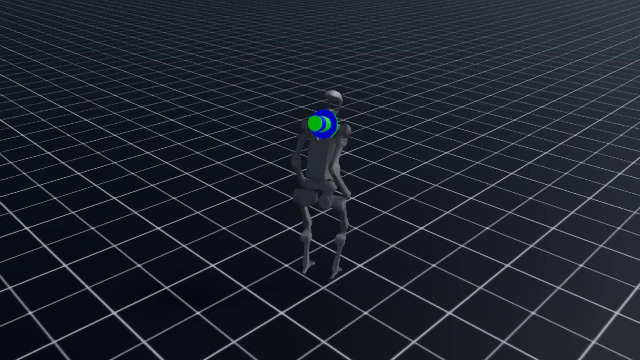
\includegraphics[width=\linewidth]{figs/5/sekaseka_seq_03.pdf}
  \end{subfigure}
  \hfill
  \begin{subfigure}[t]{0.48\linewidth}
    \centering
    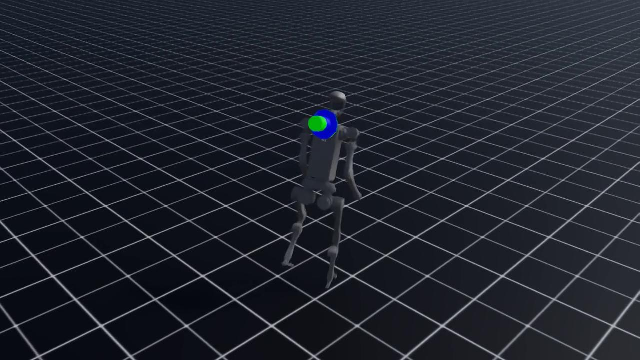
\includegraphics[width=\linewidth]{figs/5/sekaseka_seq_04.pdf}
  \end{subfigure}

  \vspace{1mm}

  \begin{subfigure}[t]{0.48\linewidth}
    \centering
    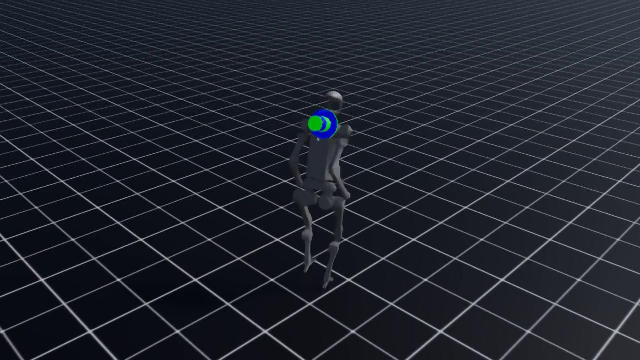
\includegraphics[width=\linewidth]{figs/5/sekaseka_seq_05.pdf}
  \end{subfigure}
  \hfill
  \begin{subfigure}[t]{0.48\linewidth}
    \centering
    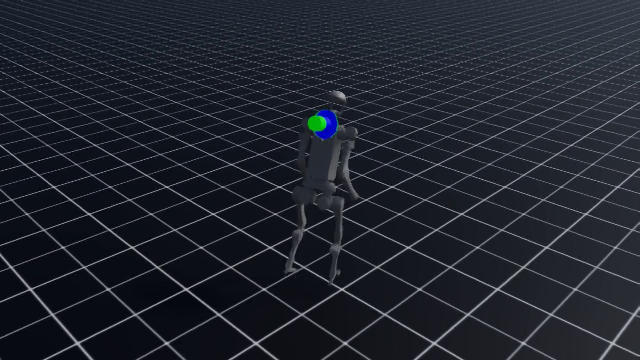
\includegraphics[width=\linewidth]{figs/5/sekaseka_seq_06.pdf}
  \end{subfigure}
  \caption{せかせかに対応する歩行}
  \label{fig:rl_sekaseka_sequence}
\end{figure}

さらに，対照学習で学習時に未使用だった未知語 7 語について，
C 条件（style\_weight=4.0）のモデルで
$v_x^{\mathrm{cmd}}=0.5$ の追加評価を行った結果を
表\ref{tab:rl_c_unknown_onom_velx}に示す．

\begin{table}[H]
  \centering
  \caption{未知語入力時の速度挙動（C 条件，速度指令値 0.5）}
  \label{tab:rl_c_unknown_onom_velx}
  \small
  \begin{tabular}{lcc} \toprule
    \textbf{オノマトペ（未知語）} & \textbf{Cmd X (m/s)} & \textbf{Vel X (m/s)} \\ \midrule
    すいすい & 0.50 & 0.4868 \\
    さっさ & 0.50 & 0.4793 \\
    のそのそ & 0.50 & 0.5109 \\
    もたもた & 0.50 & 0.5063 \\
    どすどす & 0.50 & 0.4948 \\
    ふらふら & 0.50 & 0.5228 \\
    ぐらぐら & 0.50 & 0.5100 \\ \bottomrule
  \end{tabular}
\end{table}

表\ref{tab:rl_c_unknown_onom_velx}より，未知語入力時の Vel X は 0.4793〜0.5228 に集中し，
既知語の C 条件で見られた 0.1721〜0.3179（表\ref{tab:rl_cd_onom_dynamics}）ほどの
大きな速度差は再現されなかった．
この結果から，既知語では語彙ごとの速度差が現れるのに対し，
未知語では補助速度条件側へまとまりやすいことがわかる．

\begin{table}[H]
  \centering
  \caption{オノマトペ別類似度指標（A/B/C/D，速度指令値 0.5）}
  \label{tab:rl_abcd_onom_similarity}
  \scriptsize
  \setlength{\tabcolsep}{4pt}
  \resizebox{\linewidth}{!}{%
  \begin{tabular}{lcc c c c c c c} \toprule
    \textbf{オノマトペ} &
    \multicolumn{2}{c}{\textbf{A}} &
    \multicolumn{2}{c}{\textbf{B}} &
    \multicolumn{2}{c}{\textbf{C}} &
    \multicolumn{2}{c}{\textbf{D}} \\ \cmidrule(lr){2-3}\cmidrule(lr){4-5}\cmidrule(lr){6-7}\cmidrule(lr){8-9}
    & CosR & CosC & CosR & CosC & CosR & CosC & CosR & CosC \\ \midrule
    通常 & 0.4863 & 0.4778 & 0.5002 & 0.4836 & 0.4867 & 0.4713 & 0.5559 & 0.5863 \\
    すたすた & 0.5116 & 0.5062 & 0.5283 & 0.5180 & 0.5272 & 0.5126 & 0.3767 & 0.3527 \\
    せかせか & 0.4167 & 0.4819 & 0.4236 & 0.4904 & 0.4187 & 0.4829 & 0.1998 & 0.4092 \\
    てくてく & 0.3984 & 0.4527 & 0.4034 & 0.4640 & 0.3937 & 0.4590 & 0.6321 & 0.6872 \\
    どっしどっし & 0.5255 & 0.5141 & 0.5119 & 0.5174 & 0.5142 & 0.5230 & 0.6478 & 0.7856 \\
    とぼとぼ & 0.3801 & 0.4537 & 0.3768 & 0.4585 & 0.3722 & 0.4535 & 0.5239 & 0.6555 \\
    のしのし & 0.4410 & 0.4071 & 0.4530 & 0.4124 & 0.4612 & 0.4223 & 0.5179 & 0.7452 \\
    のろのろ & 0.4055 & 0.4543 & 0.4047 & 0.4547 & 0.3996 & 0.4514 & 0.4878 & 0.6157 \\
    ぶらぶら & 0.5378 & 0.5713 & 0.5322 & 0.5653 & 0.5257 & 0.5625 & 0.6478 & 0.6547 \\
    よたよた & 0.3768 & 0.4356 & 0.3707 & 0.4302 & 0.3762 & 0.4370 & 0.6050 & 0.6044 \\
    よろよろ & 0.5288 & 0.6863 & 0.5052 & 0.6622 & 0.5071 & 0.6604 & 0.6621 & 0.6618 \\
    \bottomrule
  \end{tabular}
  }
\end{table}

表\ref{tab:rl_abcd_onom_similarity}のコサイン類似度について，
A/B/C の 3 条件では語彙ごとの CosR・CosC の値がほぼ同水準であり，
スタイル重みの増減が類似度にほとんど影響を与えていない．
一方，D 条件（style\_weight=6.0）では語彙によって値が大きく変動しており，
たとえば「どっしどっし」の CosC が他条件の約 0.52 に対して 0.79 まで上昇する一方，
「せかせか」の CosR は 0.20 まで低下するなど，語彙間のばらつきが顕著である．
このことから，スタイル重みを十分に大きくすると
類似度の分布に語彙依存の偏りが生じるが，
A/B/C の範囲では類似度指標上の差はほとんど見られなかった．


\subsubsection{スタイル識別結果（マージン混同行列）}
\label{subsubsec:rl_results_20260207}

主比較（B/C/D）のマージン混同行列を
図\ref{fig:rl_abcd_margin_b_main}，図\ref{fig:rl_abcd_margin_c_main}，
図\ref{fig:rl_abcd_margin_d_main}に示す．


\begin{figure}[H]
  \centering
  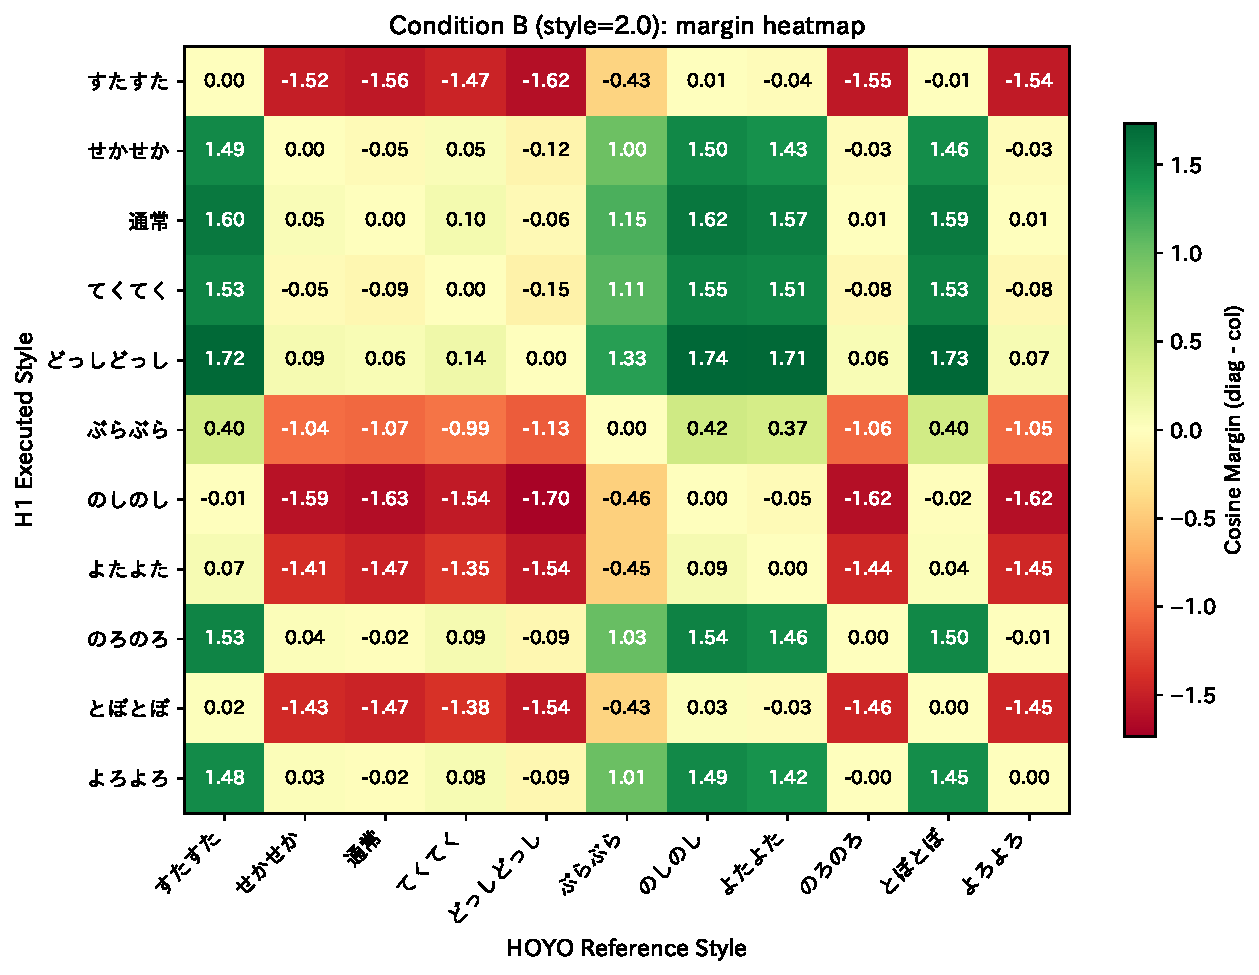
\includegraphics[width=0.8\linewidth]{figs/5/rl_abcd_B_m2999_margin_cmd05.pdf}
  \caption{B（style=2.0，速度指令値 0.5）のマージン混同行列}
  \label{fig:rl_abcd_margin_b_main}
\end{figure}

\begin{figure}[H]
  \centering
  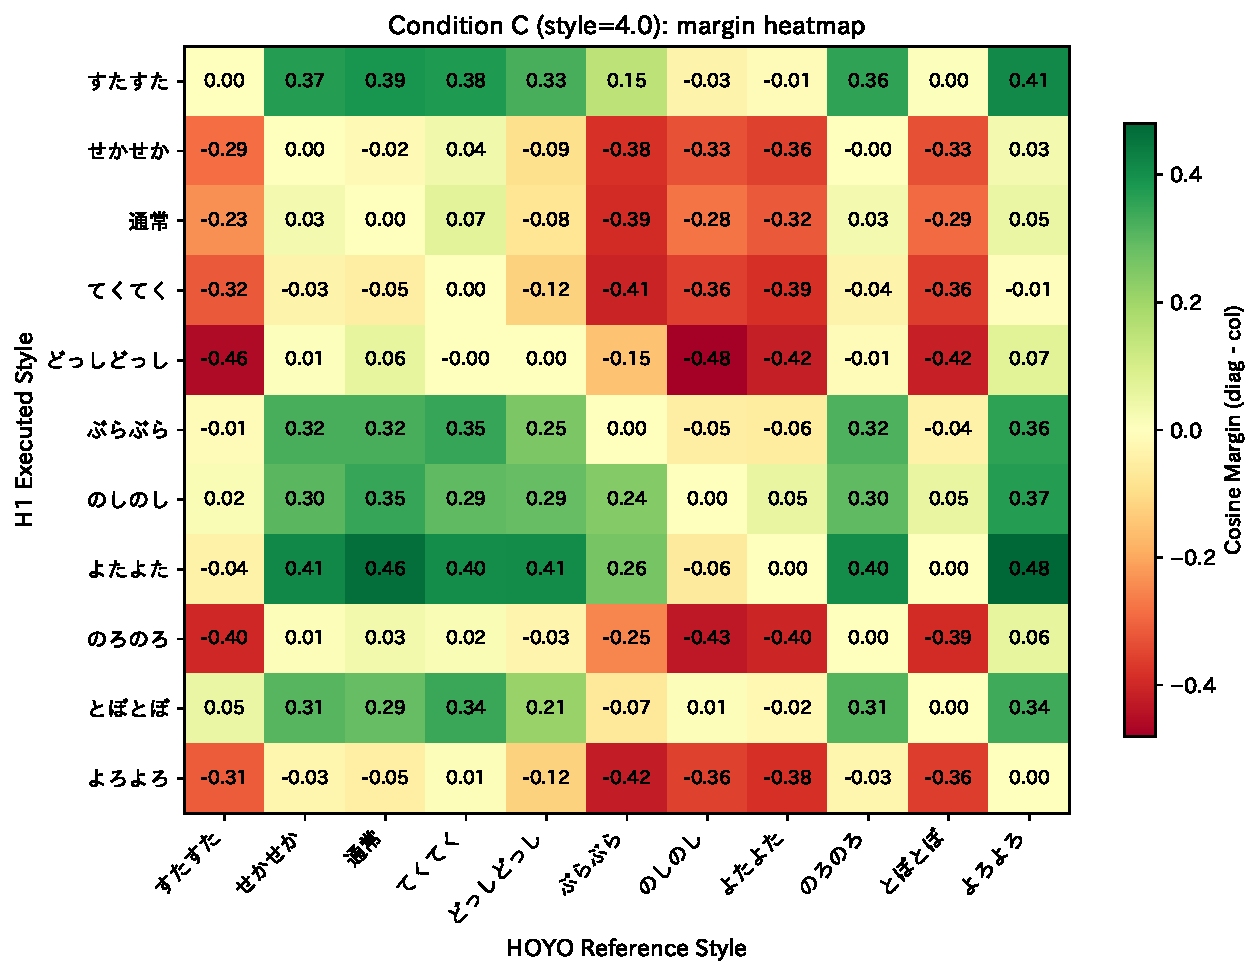
\includegraphics[width=0.8\linewidth]{figs/5/rl_abcd_C_m2999_margin_cmd05.pdf}
  \caption{C（style=4.0，速度指令値 0.5）のマージン混同行列}
  \label{fig:rl_abcd_margin_c_main}
\end{figure}

\begin{figure}[H]
  \centering
  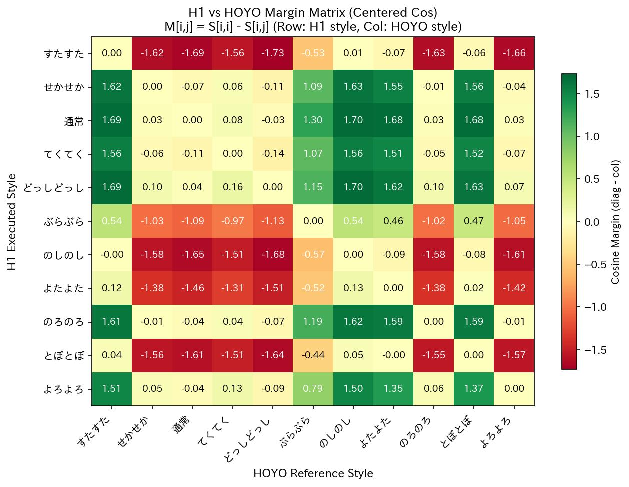
\includegraphics[width=0.8\linewidth,trim={0 0 0 6mm},clip]{figs/5/rl_20260207_style6_m2999_margin_cmd05.pdf}
  \caption{D（style=6.0，速度指令値 0.5）のマージン混同行列}
  \label{fig:rl_abcd_margin_d_main}
\end{figure}

\paragraph{マージン混同行列の読み方}\mbox{}\\

図\ref{fig:rl_abcd_margin_b_main}--\ref{fig:rl_abcd_margin_d_main}は，
実行スタイル $i$ と参照スタイル $j$ の類似度差を
$M[i,j]=S[i,i]-S[i,j]$（$S$ は centered cosine）として可視化したものである．
ここで $M[i,j]>0$ は，実行スタイル $i$ が参照 $j$ よりも自己参照 $i$ に近い
（自己ラベル優位性が保たれている）ことを意味する．
一方で $M[i,j]<0$ は，参照 $j$ の方が自己参照より近く，
スタイルの混同（誤識別）が生じていることを表す．
また，各行 $i$ における最小値は，スタイル $i$ が最も取り違えられやすい
主要な混同先に対応する．

\paragraph{条件間の傾向}\mbox{}\\

条件 C（style=4.0）は，off-diagonal 平均が $-0.0002$ と 0 付近に留まり，
自己優位性 $S[i,i]-S[i,j]$ が小さい状態が多く確認された．
これは自己参照と他参照の差が縮小し，
埋め込み空間上でスタイル識別の分離が弱いことを示唆する．
一方で条件 B（style=2.0）および条件 D（style=6.0）は，
off-diagonal 平均がそれぞれ $+0.0084$，$+0.0091$ と正側を示し，
相対的には自己ラベル優位性が回復している．
ただし，すべてのスタイルで一様に改善するわけではなく，
負側の成分が残る行も確認されるため，識別構造は依然として安定していない．

\paragraph{主要な混同先の集中と解釈}\mbox{}\\

主要な混同先の分布に着目すると，
条件 B と条件 D では多くの行において混同先が「どっしどっし」列に集中した
（いずれも 10/11 行）．
これは，複数スタイルの実行軌道が参照「どっしどっし」に相対的に近づく，
あるいは「どっしどっし」参照が他スタイルと共有する歩容成分を強く含むことで
埋め込み空間上のハブ（吸引先）として機能している可能性を示す．
一方で条件 C では混同先が「ぶらぶら」（5/11）と「のしのし」（4/11）に分散しており，
特定参照への一方向な収束よりも，
全体として識別境界が曖昧化している状態が示唆される．
要因分析は第\ref{chap:考察}章で述べる．

\subsubsection{位相シフトに対する cos 類似度の感度}
\label{subsubsec:rl_results_phase_shift}

スタイル報酬で用いる cos 類似度が時間位相のずれにどの程度敏感かを確認するため，
補助評価を実施した．
この評価は上記表とは異なる学習モデルで実施したため，絶対値の比較ではなく
位相シフトに対する変動幅の確認を目的とする．

具体的には，H1 側の motion を長めに保持し，HOYO 教師 motion を固定したうえで，
H1 側の時間窓のみをシフトさせて cos 類似度（CosR）を再計算した．
各オノマトペに対して CosR の最小値・最大値・変動幅（range）を表\ref{tab:rl_phase_shift_cos}に示す．

\begin{table}[H]
  \centering
  \caption{位相シフト時の CosR 変動（補助評価，別モデル）}
  \label{tab:rl_phase_shift_cos}
  \begin{tabular}{lccc} \toprule
    \textbf{オノマトペ} & \textbf{CosR\_min} & \textbf{CosR\_max} & \textbf{range} \\ \midrule
    すたすた & 0.387 & 0.394 & 0.007 \\
    のろのろ & 0.467 & 0.473 & 0.006 \\
    とぼとぼ & 0.511 & 0.515 & 0.004 \\
    よたよた & 0.581 & 0.585 & 0.004 \\
    よろよろ & 0.651 & 0.655 & 0.004 \\
    通常 & 0.572 & 0.574 & 0.002 \\
    せかせか & 0.230 & 0.232 & 0.002 \\
    どっしどっし & 0.659 & 0.661 & 0.002 \\
    ぶらぶら & 0.618 & 0.620 & 0.002 \\
    てくてく & 0.647 & 0.647 & 0.000 \\
    のしのし & 0.479 & 0.479 & 0.000 \\ \bottomrule
  \end{tabular}
\end{table}

表\ref{tab:rl_phase_shift_cos}より，位相シフトによる CosR の変動幅は最大でも 0.007 であった．
この結果から，本実験範囲ではスタイル報酬計算時の位相ずれの影響は小さく，
厳密な位相合わせを行わなくても評価値は大きく変化しないことが示唆される．
したがって，現段階では位相同期よりも，表現分離や報酬重み設計の改善を優先すべきである．

\subsubsection{オノマトペ別解析（速度・cos類似度・関節誤差）}
\label{subsubsec:rl_results_20260208_residual}

本研究の主要分析粒度はオノマトペ別である．
residual\_scale=0.3 条件と residual\_scale=0.8 条件を，
同一の対照学習のbest modelを用いて，
同じ $v_x^{\mathrm{cmd}}=0.3$ で比較した結果を
表\ref{tab:rl_20260208_residual_metrics}に示す．

\begin{table}[H]
  \centering
  \caption{residual\_scale 比較（オノマトペ別，速度指令値 0.3）}
  \label{tab:rl_20260208_residual_metrics}
  {\scriptsize
  \begin{tabular}{lcccccc} \toprule
    \textbf{オノマトペ} & \textbf{$v_x$ (0.3)} & \textbf{$v_x$ (0.8)} & \textbf{cos(C) (0.3)} & \textbf{cos(C) (0.8)} & \textbf{Err (0.3)} & \textbf{Err (0.8)} \\ \midrule
    通常 & 0.3367 & 0.0421 & 0.5816 & 0.5736 & 3.3650 & 3.6271 \\
    すたすた & 0.3069 & 0.0398 & 0.3293 & 0.3228 & 3.9833 & 4.5572 \\
    せかせか & 0.3176 & 0.0433 & 0.3934 & 0.3841 & 3.1023 & 3.6557 \\
    てくてく & 0.3354 & 0.0294 & 0.6767 & 0.6743 & 3.5465 & 3.7470 \\
    どっしどっし & 0.3470 & 0.0309 & 0.7782 & 0.7725 & 3.2033 & 3.6833 \\
    とぼとぼ & 0.3368 & 0.0336 & 0.6715 & 0.6647 & 4.2531 & 4.4908 \\
    のしのし & 0.3354 & 0.0325 & 0.7501 & 0.7453 & 3.9140 & 4.5525 \\
    のろのろ & 0.3547 & 0.0336 & 0.6280 & 0.6210 & 2.9790 & 3.3766 \\
    ぶらぶら & 0.3342 & 0.0330 & 0.6765 & 0.6638 & 4.0337 & 4.1634 \\
    よたよた & 0.3505 & 0.0341 & 0.6281 & 0.6217 & 4.2813 & 4.3420 \\
    よろよろ & 0.3544 & 0.0350 & 0.6827 & 0.6764 & 3.3834 & 3.5048 \\
    \bottomrule
  \end{tabular}
  }
\end{table}

\begin{figure}[H]
  \centering
  \begin{subfigure}[t]{0.49\linewidth}
    \centering
    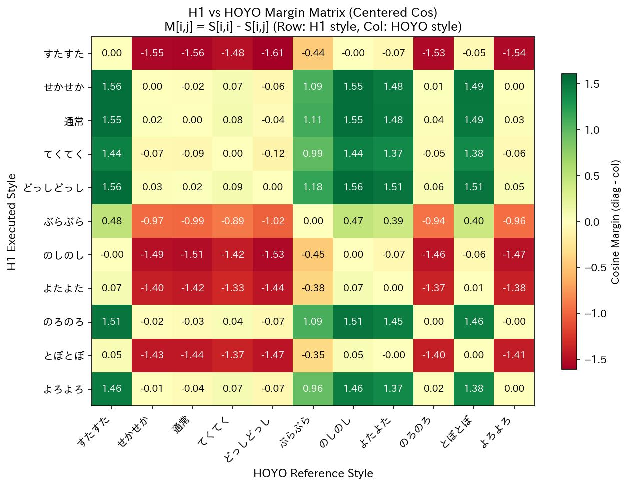
\includegraphics[width=\linewidth]{figs/5/rl_20260207_res03_style_m2999_margin_cmd03.pdf}
    \caption{residual=0.3}
  \end{subfigure}
  \hfill
  \begin{subfigure}[t]{0.49\linewidth}
    \centering
    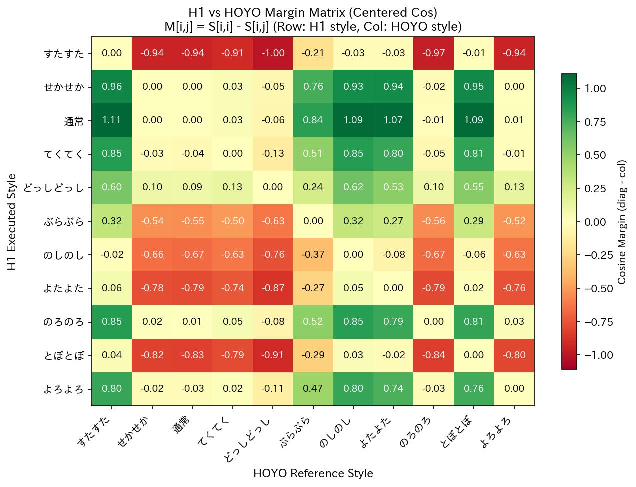
\includegraphics[width=\linewidth]{figs/5/rl_20260208_res08_bestmodel_margin_cmd03.pdf}
    \caption{residual=0.8（対照学習のbest model）}
  \end{subfigure}
  \caption{residual\_scale 比較（速度指令値 0.3）のマージン混同行列}
  \label{fig:rl_20260208_residual_margin}
\end{figure}

residual\_scale=0.3 と 0.8 の比較により，11 オノマトペそれぞれの速度，
cos 類似度，関節誤差を同一条件で横断的に確認した．
全体傾向としては，residual\_scale=0.3 の方が前進維持（速度低下の抑制）・cos 類似度の両面で一貫して高く，
対照学習のbest model下の residual\_scale=0.8 条件では速度低下と関節誤差増大が同時に生じた．


未解決課題と要因分析は，第\ref{chap:考察}章で述べる．
